%********************************************************************
% Appendix
%*******************************************************
% If problems with the headers: get headings in appendix etc. right
%\markboth{\spacedlowsmallcaps{Appendix}}{\spacedlowsmallcaps{Appendix}}
\chapter{Experimental Realization of Bell's Inequality with the Quantenkoffer}
\label{appendexA:Bell_exp_quCASE}

\section{Necessary Components}

\begin{itemize}
	\item Quantenkoffer
	\item 4 Periscopes
	\item 2 Polarizers
\end{itemize}

\section{Experimental description}

\begin{itemize}
	\item \textbf{Preperation: }
	Please plug in the two polarizers as shown in fig below. The source has to be adjusted to obtain the best possible entanglement with the periscopes.
	\item \textbf{Bell experiment: }
	Set the polarizers to one of the 16 settings listed on the worksheet by touching the respective polarizer and set it to the "Follow" Mode. In the LineView, you can then read off the coincidence count rate for that setting. After you've done that for all 16 settings, you can calculate the S-value.
	\item \textbf{Other States: }
	For comparison of the results with other input states, try setting the wave plate in the source to another angle. By doing that you can either produce another entangled state (set to M), but you can also produce product states (set to H or V). With these states, you can repeat all measurements. For convenience, there is also the BellView, in which you can measure all 16 settings in a quick and easy way. Depending on the value for the integration time, the measurement is going to be either faster or more precise
\end{itemize}

\begin{figure}[H]
	\centering
	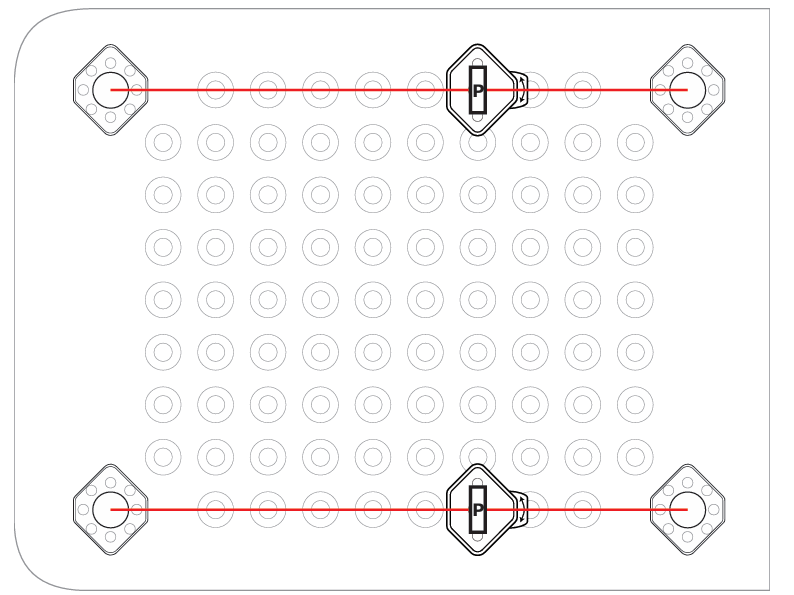
\includegraphics[width=0.70\textwidth]{gfx/diagrams/bell_qucase.png}
	\caption{ For the Bell Experiment, put one polarizer in each beam path. You then set the polarizers to different angles and record the coincidence count rate for each setting} 
	\label{fig:A.2.1}
\end{figure}

\begin{figure}[H]
	\centering
	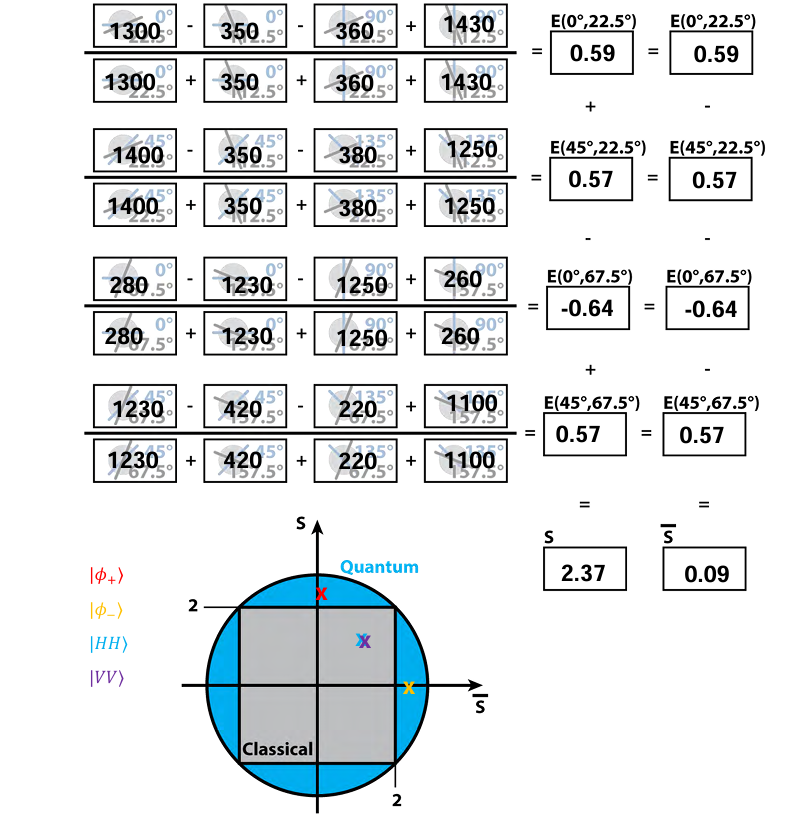
\includegraphics[width=0.60\textwidth]{gfx/diagrams/angles_worksheet.png}
	\caption{Worksheet} 
	\label{fig:A.2.2}
\end{figure}

\chapter{quEDU Python GUI Software - Setup}
\label{appendixB: qudi_installation}

\section{Based on Python Version 3.10}

The quEDU(-NV) Python software is developed using Python Version 3.10, with the objective of ensuring compatibility with the qudi-Framework. However, it is also capable of being executed as a standalone application.

\begin{itemize}
	\item \textbf{Install Python 3.10}
\end{itemize}

\section{Update installation tools}

\begin{itemize}
	\item \textbf{python.exe -m pip install --upgrade pip setuptools wheel}
	\item \textbf{Also update basic packages like numpy, pip, ... etc}
\end{itemize}

\section{qudi framework}

If you like to use the qudi framework, it’s best to create an virtual python environment venv, based on python 3.10, in a folder you like for to install the qudi framwork in:

\begin{itemize}
	\item \textbf{virtualenv venv --python=python3.10}
\end{itemize}

Activate this virtual python environment :
 
\begin{itemize}
 	\item \textbf{ ./\/venv/\/Scripts/\/activate(.bat or .ps1)}
\end{itemize}
 
You’ve got the promt :
 
\begin{itemize}
 	\item \textbf{(venv)}
\end{itemize}
  
Update also the installation tools in the virtual python environment :
  
\begin{itemize}
	\item \textbf{(venv) python.exe -m pip install --upgrade pip setuptools wheel}
\end{itemize}
 
There are several QUDI frameworks, also old and pure ones, in the Web, but the best package seems to come from the IQO institut of Ulm  :

\begin{itemize}
	\item \textbf{ (venv) pip install qudi\_iqo\_modules}
\end{itemize}

Copy the quEDU Python Software Files into the qudi lib folder. Change the path inside of the install batch file and call:

\begin{itemize}
	\item \textbf{install\_modules.bat}
\end{itemize}

Some modules should be installed in qudi folders, like GUI, Logic, Interface and Hardware, but in qutools subfolder.

Copy the quEDU.cfg file to the place, where qudi takes this files (User area)  :

\begin{itemize}
	\item \textbf{copy quEDU.cfg ...}
\end{itemize}

Call qudi framework inside of the virtual environment and load the quEDU.cfg file:

\begin{itemize}
	\item \textbf{ (venv) qudi}
\end{itemize}

\section{Continue without qudi framework and virtual python environement}

Without qudi installation, you need additional python libs (numpy, pyqtgraph, PySide2) for the standalone GUI. They are listed in the requirement file. You can install these libs by taking this requirement file

\begin{itemize}
	\item \textbf{pip install -r requirements.txt}
\end{itemize}

\section{Start quEDU Python Software}

In qudi the quEDU Python Modules are started inside of the qudi framework.As standalone App, you call the quEDU\_Main.py module. This modules do some 
configuration, which are done in qudi by the qudi framework

\begin{itemize}
	\item \textbf{py quEDU\_Main.py}
\end{itemize}